\chapter{Additional graphs and analysis}

\section{Sample data from dataset}
\begin{table}[ht]
    \captionsetup{font=small}
    \centering
    \begin{tabularx}{\textwidth}{|l|X|c|c|l|}
        \hline
        \rowcolor[gray]{0.7}
        \textbf{id} & \textbf{text}                                               & \textbf{binarylabel} & \textbf{multilabel} & \textbf{domain} \\
        \hline
        1.20E+17    & asus g60 series . bought it to play games but guess not bf3 & 1                    & 1                   & electronics     \\
        \hline
        4.88E+17    & love this trimmer ! making the sidewalk look sharp <url>    & 0                    & 0                   & other           \\
        \hline
    \end{tabularx}
    \caption{Sample data from \cite{jinModelingSeverityComplaints2021}. The \texttt{binarylabel} represents the label for complaints with 1 indicating the tweet is a complaint. Columns \texttt{id} and \texttt{multilabel} are not used for the experiments}
    \label{tab: apdx_sample_data}
\end{table}

\section{Breakdown of tweets in full dataset}
\begin{table}[ht]
    \captionsetup{font=small}
    \centering
    \begin{tabularx}{\textwidth}{|X|c|c|c|}
        \hline
        \rowcolor[gray]{0.7}
        \textbf{Domains}            & \textbf{Complaints}   & \textbf{Non-Complaints} & \textbf{Total Tweets} \\
        \hline
        Apparel                     & 145 \small{(55.3\%)}  & 117 \small{(44.7\%)}    & 262 \small{(7.6\%)}   \\
        \hline
        Cars                        & 68 \small{(73.1\%)}   & 25 \small{(26.9\%)}     & 93 \small{(2.7\%)}    \\
        \hline
        Electronics                 & 176 \small{(60.7\%)}  & 114 \small{(39.3\%)}    & 290 \small{(8.4\%)}   \\
        \hline
        Food \& Beverage            & 92 \small{(72.4\%)}   & 35 \small{(27.6\%)}     & 127 \small{(3.7\%)}   \\
        \hline
        Other                       & 95 \small{(74.2\%)}   & 33 \small{(25.8\%)}     & 128 \small{(3.7\%)}   \\
        \hline
        Retail                      & 122 \small{(61.9\%)}  & 75 \small{(38.1\%)}     & 197 \small{(5.7\%)}   \\
        \hline
        Services                    & 204 \small{(60.9\%)}  & 131 \small{(39.1\%)}    & 335 \small{(9.7\%)}   \\
        \hline
        Software \& Online Services & 192 \small{(65.1\%)}  & 103 \small{(34.9\%)}    & 295 \small{(8.6\%)}   \\
        \hline
        Transport                   & 138 \small{(55.9\%)}  & 109 \small{(44.1\%)}    & 247 \small{(7.2\%)}   \\
        \hline
        \rowcolor[gray]{0.9}
        \textbf{Sub-total}          & 1232 \small{(62.4\%)} & 742 \small{(37.6\%)}    & 1974                  \\
        \hline
        \hline
        Random Reply                & 0 \small{(0\%)}       & 739 \small{(100\%)}     & 739 \small{(21.4\%)}  \\
        \hline
        Random Tweet                & 0 \small{(0\%)}       & 736 \small{(100\%)}     & 736 \small{(21.3\%)}  \\
        \hline
        \hline
        \textbf{Total}              & 1232 \small{(63\%)}   & 739 \small{(37\%)}      & 1971                  \\
        \hline
    \end{tabularx}
    \caption{The nine domains and the distribution of tweets that are complaints and those that are not. The percentages indicate how the splits are distributed \cite{preotiuc-pietro_automatically_2019}.}
    \label{tab: fulldataset_breakdown}
\end{table}


\section{Token distribution after tokenization}
\label{sec: apdxa_token_dist}
The graphs in Figure \ref{fig: apdxa_tokens} show the distribution of token size for tweets from the full dataset for each of the models based on the tokenizer they use. The graph for BERT base uncased is in Chapter 3, Figure \ref{fig: bef_aft_token}.
\begin{figure}[htbp]
    \centering
    \captionsetup{font=small}
    \begin{subfigure}[b]{0.48\textwidth}
        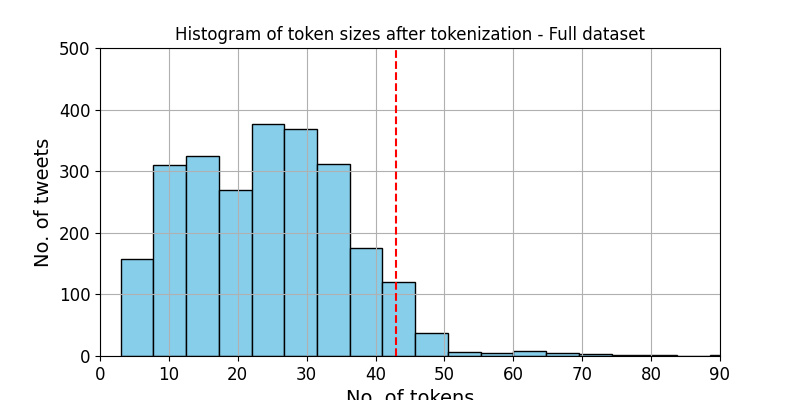
\includegraphics[width=\textwidth]{figures/token_pp_hist_albert-base-v2.png}
        \caption{Albert base}
        \label{fig: token_pp_hist_albert}
    \end{subfigure}
    \hfill
    \begin{subfigure}[b]{0.48\textwidth}
        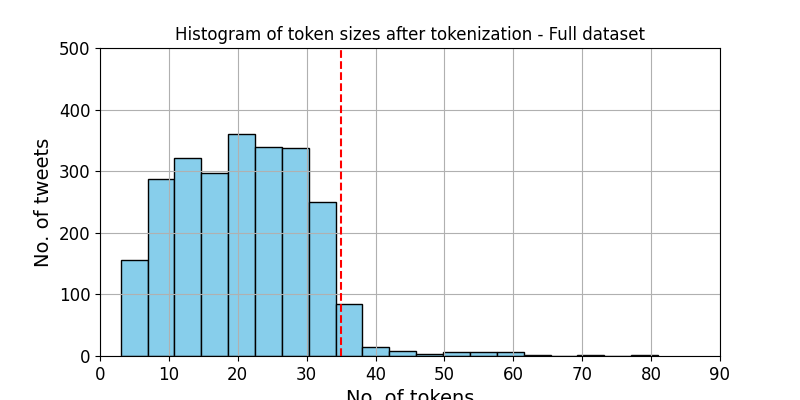
\includegraphics[width=\textwidth]{figures/token_pp_hist_vinai-bertweet-base.png}
        \caption{BERTweet}
        \label{fig: token_pp_hist_bertwteet}
    \end{subfigure}
    \begin{subfigure}[b]{0.48\textwidth}
        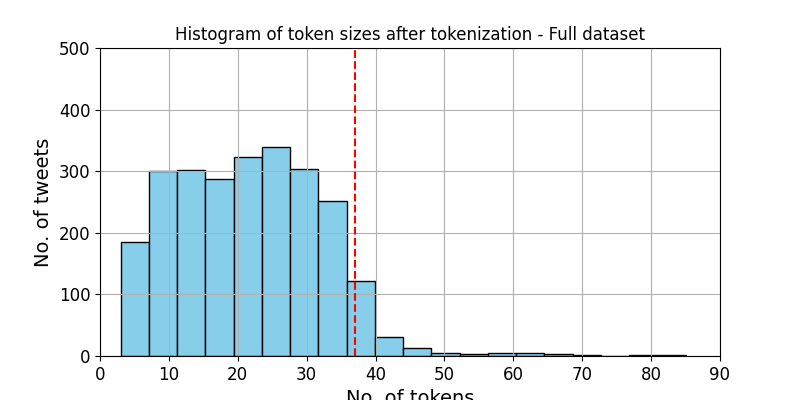
\includegraphics[width=\textwidth]{figures/token_pp_hist_prajjwal1-bert-tiny.png}
        \caption{BERT tiny}
        \label{fig: token_pp_hist_tiny}
    \end{subfigure}
    \hfill
    \begin{subfigure}[b]{0.48\textwidth}
        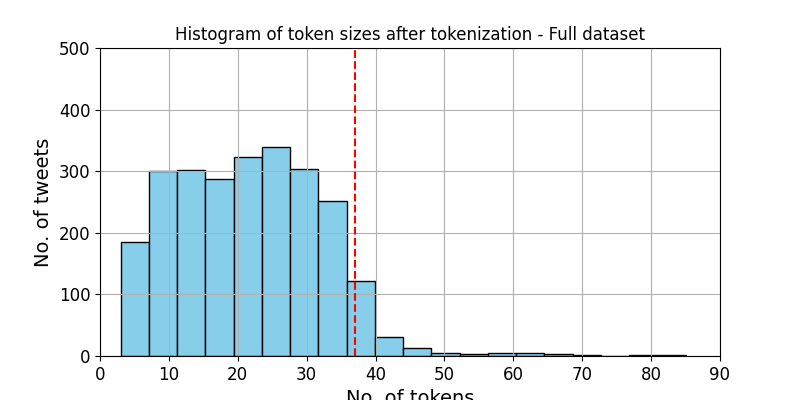
\includegraphics[width=\textwidth]{figures/token_pp_hist_distilbert-base-uncased.png}
        \caption{DistilBERT base uncased}
        \label{fig: token_pp_hist_distilbert}
    \end{subfigure}
    \begin{subfigure}[b]{0.48\textwidth}
        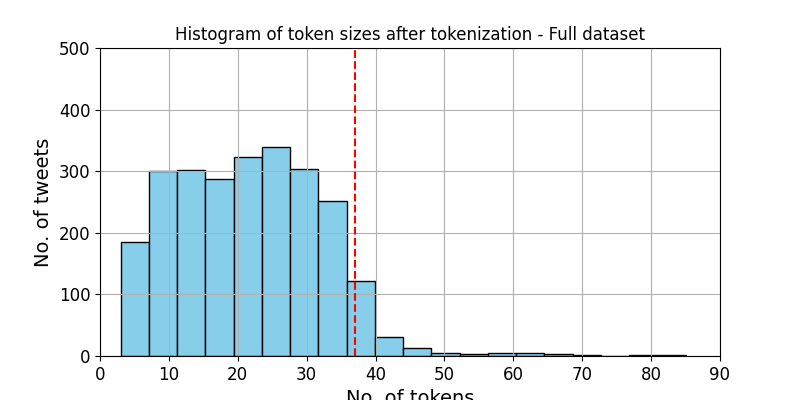
\includegraphics[width=\textwidth]{figures/token_pp_hist_google-mobilebert-uncased.png}
        \caption{MobileBERT uncased}
        \label{fig: token_pp_hist_mobile}
    \end{subfigure}
    \hfill
    \begin{subfigure}[b]{0.48\textwidth}
        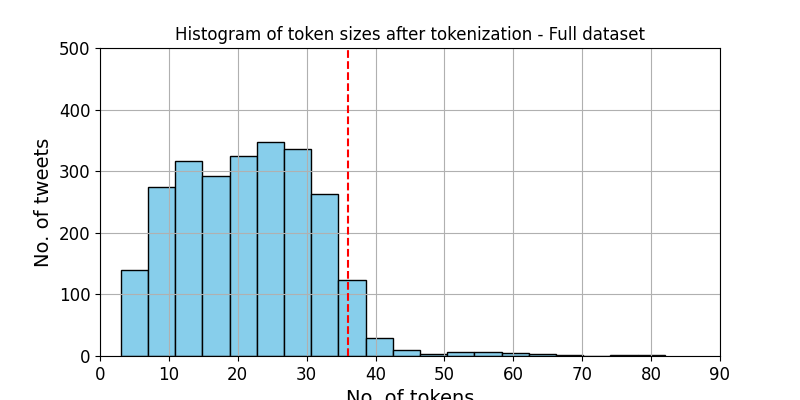
\includegraphics[width=\textwidth]{figures/token_pp_hist_roberta-base.png}
        \caption{Roberta base}
        \label{fig: token_pp_hist_roberta}
    \end{subfigure}
    \caption{The token count distribution for the full dataset of 3,449 tweets for all models.}
    \label{fig: apdxa_tokens}
\end{figure}